\chapter{Critical period plasticity in tumor necrosis factor-\textalpha{}-deficient mice}

\section{Overview}
\newrefsection

Early experience shapes sensory representations in a critical period of heightened plasticity. This adaptive process is thought to involve both Hebbian and homeostatic synaptic plasticity. Although Hebbian plasticity has been investigated as a mechanism for cortical map reorganization, less is known about the contribution of homeostatic plasticity. We investigated the role of homeostatic synaptic plasticity in the development and refinement of frequency representations in the primary auditory cortex using the tumor necrosis factor-\textalpha{} (TNF-\textalpha{}) knockout (KO) mouse, a mutant with impaired homeostatic but normal Hebbian plasticity. Our results indicate that these mice develop weaker tonal responses and incomplete frequency representations. Rearing in a single-frequency revealed a normal expansion of cortical representations in KO mice. However, TNF-\textalpha{} KO mice lacked homeostatic adjustments of cortical responses following exposure to multiple frequencies. Specifically, while this sensory over-stimulation resulted in competitive refinement of frequency tuning in wild-type controls, it broadened frequency tuning in TNF-\textalpha{} KO mice. Our results suggest that homeostatic plasticity plays an important role in gain control and competitive interactions in sensory cortical development.

\section{Introduction}

Rodent auditory cortex undergoes rapid maturation during early postnatal development, as manifested by the emergence and refinement of cortical sound representations (\cite{Zhang2001, Chang2005, DeVillers-Sidani2007, Insanally2009}). This process is shaped by acoustic experience in a “critical period” of heightened plasticity (\cite{DeVillers-Sidani2007}). Recent studies indicate that the auditory cortex is sensitive to different sound features across developmental stages within the critical period (\cite{Insanally2009, Popescu2010}). For example, early critical period experience shapes the cortical frequency map (\cite{DeVillers-Sidani2007, Insanally2009}), whereas later critical period experience shapes frequency modulation selectivity (\cite{Insanally2009, Insanally2010}). In addition, the characteristics of developmental plasticity depend on the properties of the acoustic input (\cite{Chang2003, Zhou2008}). While exposure to a pulsed tone repeated at an ethological rate results in enlarged representation of the tone, exposure to the same tone repeated at a higher or lower rate does not (\cite{Kim2009}). Early experience also alters sound perception and perceptual behaviors in ways consistent with the reorganized sound representation in the auditory cortex (\cite{Han2007}). Thus, multifaceted auditory cortical plasticity may be a useful model to investigate molecular/cellular mechanisms of sensory development and pathologies of developmental sensory disorders.

Refinement of sensory representations during the critical period is believed to be mediated by experience-dependent synaptic plasticity (\cite{Dan2006, Feldman2009}). Sensory experience is shown to engage at least two types of synaptic plasticity in sensory cortex: Hebbian and homeostatic synaptic plasticity (\cite{Desai2002, Fu2002, Heynen2003, Crozier2007, Goel2007, Maffei2008}). Hebbian plasticity, which includes long-term potentiation (LTP) and long-term depression (LTD), and spike-timing­-dependent plasticity, rapidly alters the strength of individual synapses in an input-specific manner (\cite{Zhang1998, Abbott2000, Malenka2004, Dan2006}). In contrast, homeostatic plasticity globally or locally adjusts synaptic strength onto the neuron following prolonged changes in neuronal activity level (\cite{Davis2001, Burrone2003, Turrigiano2004, Hou2008}). An important difference between Hebbian and homeostatic plasticity is how they adjust synaptic strength when a neuron is overstimulated. Hebbian plasticity stengthens excitatory synapses when pre- and post-synpatic neurons are coactivated and weakens excitory synapses when pre-synaptic neuron is activated alone. In the sensory cortex, repeated activation of a cortical neurons by a stimulus may engage Hebian plasticity to strengthen excitatory connections, resulting in enhanced cortical responses to the stimulus (\cite{Zhang2001}). This change is, at least partly, mediated by enhanced excitatory responses (\cite{Froemke2007, Sun2010}). Sensory deprivation may reduce cortical responses to the deprived sensory organ through Hebbian synaptic depression (\cite{Heynen2003}). In contrast, homeostatic plasticity should weaken exciatory synpases and strengthen inhibitory synpases onto a neuron when the neuron is over-stimulated. Thus, through homeostatic plasticity, repeated sensory stimulation could lead to weakened cortical responses (\cite{Condon1991, Pienkowski2012}).

While Hebbian plasticity in sensory development has been investigated extensively (\cite{Feldman2009}), the role of homeostatic plasticity has been investigated only recently (\cite{Mrsic-Flogel2007}). Experimental findings in the visual and somatosensory systems indicate that a form of homeostatic plasticity is involved in ocular dominance shifts during the critical period but not in adulthood (\cite{Kaneko2008, Ranson2012}). Following monocular deprivation, Hebbian LTD causes a reduction in responses to stimulation of the deprived eye and subsequent homeostatic plasticity results in competitive enhancement of responses to the open eye (\cite{Frenkel2004, Kaneko2008, Ranson2012}). While these findings provide convincing evidence of a role for homeostatic plasticity in this particular experimental paradigm, it remains to be determined whether and how it may be involved in other forms of developmental plasticity both within the visual system and in other sensory systems.

Earlier studies have taken advantage of strains of mice that are deficient in homeostatic plasticity (\cite{Kaneko2008, Ranson2012}). For example, the tumor necrosis factor-\textalpha{} (TNF-\textalpha{}) knockout (KO) mouse, which is deficient in homeostatic up-regulation of excitatory synaptic transmission and downregulation of inhibitory transmission in response to activity blockade (\cite{Stellwagen2006, Kaneko2008}), exhibits normal monocular deprivation-induced loss of deprived-eye responses in the initial stages of ocular dominance shift but not the subsequent increase in open eye responses (\cite{Kaneko2008}).

In the present study, we examined the role of homeostatic plasticity in the development and plasticity of sound representations in TNF-\textalpha{} KO mouse. KO mice raised in the typical animal room environment had highly variable cortical frequency maps, often showing incomplete representation of the mouse-hearing frequency range. Although both WT and KO mice developed enlarged representations of a repeatedly exposed tone, they showed opposite effects as a result of multi-frequency exposure---narrowed frequency tuning in WT mice and broadened frequency tuning in KO mice. These results suggest that homeostatic plasticity may be involved in normal development and competitive refinement of acoustic representation in the primary auditory cortex.

\section{Methods}

\subsection{Acoustic Exposure}

All procedures used in this study were approved by the UC Berkeley Animal Care and Use Committee. Litters of juvenile TNF-\textalpha{} KO mice (KO) and corresponding C57BL/6 wild-type mice (WT) from the Jackson Laboratory together with the nursing females were assigned to one of the 3 groups---a tone-exposure group, an enriched environment group, and a control group. The two experimental groups were repeatedly exposed to 1 s long trains of 6 tone pips (100 ms, 65 dB sound pressure level (SPL), 5-ms on and off cosine-squared ramps), with one train occurring every 2 s. The frequency of the tone pips within a train was the same, and was either fixed at 25 kHz for the tone-exposure group or randomly chosen from a continuum that ranged from 4 to 45 kHz for the enriched environment group. For this group, the acoustic power of the exposure sounds was uniformly distributed along the logarithmic frequency axis from 4 to 45 kHz (e.g. the power in the 4-8 kHz range is the same as in 8-16 kHz range). Sounds were generated with a National Instrument I/O card at a sampling rate of 200 kHz, amplified, and played through a calibrated speaker in a sound-attenuation chamber where the animals were housed. The sound exposure started on postnatal day 9 (P9) and ended immediately before electrophysiological examination was conducted, typically on P19 to P21. Both sound exposed groups were compared with the control group, which were maintained in regular animal rooms and were mapped during the same period as the 2 experimental groups. The acoustic environment of the animal room is dominated by ambient low-level noise. Constant, broadband sounds at such low levels cannot mask sensory input. In addition, unmodulated sounds are ineffective in shaping sensory representations (\cite{Kim2009}).

\subsection{Electrophysiological Recording Procedure}

The primary auditory cortex (AI) in na\"ive and sound-exposed KO and WT mice was mapped as previously described (\cite{Kim2009}). Mice were anesthetized with ketamine (100 mg/kg, IP) and xylazine (10 mg/kg, IP), and placed on a homeothermic heating pad at 36.5$^\circ$C (Harvard Apparatus) in a sound attenuation chamber. The head was secured with a custom head-holder that left the ears unobstructed. The right auditory cortex was exposed and kept under a layer of silicone oil to prevent desiccation. Multi-unit activity was evenly sampled from primary auditory cortex. AI in both WT and KO mice was found consistently underneath the caudal half of the temporal-parietal bone suture. It can be identified by its tonotopic orientation---higher frequencies are represented more rostrally and slightly more dorsally. Other auditory cortical fields have different tonotopic orientations (\cite{Guo2012}). The border of AI was defined by unresponsive sites or sites whose CFs were incongruent with the AI tontopic gradient. Because KO mice tended to have incomplete representations of low and high frequencies (Fig. 1), we carefully searched for those representations near the rostral and caudal ends of AI in both WT and KO mice, while maintaining the same sampling density. Typical sampling extent and density is shown in the map from animal 3 in Figure 1A. Neural responses were recorded using tungsten microelectrodes (FHC) at a depth of 400-450 \textmu m, presumably from the thalamorecipient layer. Responses to 25-ms tone pips of 41 frequencies (4-64 kHz, 0.1 octave spacing) and 8 sound pressure levels (10-80 dB SPL, 10-dB steps) were recorded to reconstruct the frequency-intensity-receptive field. A Tucker-Davis Technologies coupler model electrostatic speaker was used to present all acoustic stimuli into the left ear (contralateral to the recorded cortical hemisphere). Each frequency-intensity combination was repeated 3 times.

\begin{figure}
	\centering
		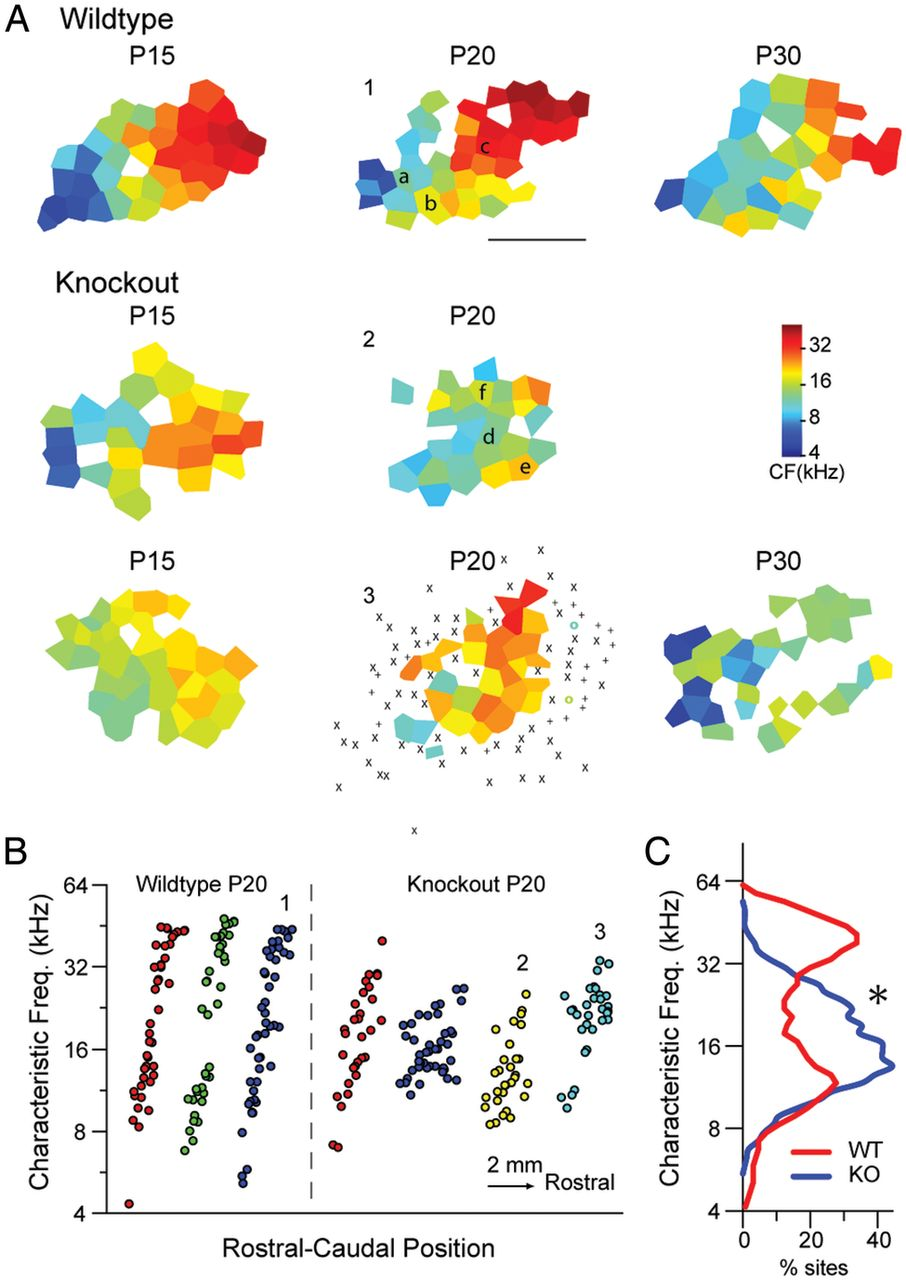
\includegraphics[width=4in]{images/C3F1}
	\begin{changemargin}{1in}{1in}
	\footnotesize{Figure 1. Development of cortical frequency map is impaired in TNF-\textalpha{} KO mice. (A) Example frequency maps at P15, P20, and P30 from WT and TNF-\textalpha{} KO mice. Receptive fields recorded at locations a-f are shown in Figure 2. The scale bar is 1 mm long and applies to all maps. The map from animal number 3 shows typical sampling density and extent. +, unresponsive sites where neural responses were visually examined but not recorded; x, unresponsive sites where neural responses were recorded; o, responsive sites where CF was incongruent with AI tonotopy. (B) Representative distributions of neuronal CFs along rostral-caudal axis recorded from 8 animals at P20. Note that the KO maps had more sites without an identifiable receptive field as indicated by the white regions within the maps. In addition, the represented frequency ranges were narrower and more variable in the KO mice. Plots marked with 1-3 were from the three P20 animals whose maps are shown in (A). (C) Percent of sites representing frequencies ($\pm0.3$ octaves). * indicates a statistically significant difference.}
	\end{changemargin}
\end{figure}

\subsection{Data Analysis}

The receptive fields and response properties were isolated using custom-made programs. First, the peri-stimulus time histogram (PSTH) was generated from responses to all 328 (41 frequencies $\times$ 8 intensities) tone pips, with 1-ms bin size (Fig. 4E). The mean firing rate was calculated for each bin and smoothed with a 5-point mean filter. The multiunit spontaneous firing rate was taken as the mean firing rate in the 50-ms window prior to stimulus onset. Peak latency was defined as the time to the peak PSTH response between 7 and 50 ms after the stimulus onset. The response window was defined as the period encompassing the PSTH peak, in which the mean firing rate in every bin was higher than baseline firing rate. The onset latency was defined at the onset of the response window. The tone-evoked response was measured as the maximum firing rate within the response window. Spikes that occurred within the response window were counted to reconstruct the receptive field.

The tuning curve contour was determined using a smoothing and thresholding algorithm. The response magnitude was plotted in the frequency-intensity space, and smoothed with a 3$\times$3 mean filter (see Fig. 2B for examples). It was then thresholded at 28\% of the maximum value of the smoothed response magnitude. Response areas smaller than 5 pixels were removed. The contour of the suprathreshold area was defined as the tuning curve. The raw responses in the suprathreshold area were defined as the isolated receptive field. The threshold of the neuron was the lowest sound level that elicited responses in the isolated receptive field. The characteristic frequency (CF) of a neuron was defined as the center of mass of the isolated receptive field for the two lowest suprathreshold sound levels. The center of mass CF was defined as $\sum{(R_i \times f_i)}/\sum{R_i}$, in which $R_i$ is the response magnitude to the $i$th tone with frequency $f_i$, and responses were collapsed across the two sound levels. The maximum RF response was the maximum number of spikes activated by a single frequency-intensity combination. The mean RF response was the mean number of spikes for all frequency-intensity combinations within the receptive field. Tuning bandwidth (BW) was defined as the frequency extent in octaves of the receptive field at the specified intensity. We quantified BW at 80, 70, and 60 dB SPL, but not at lower SPLs because many neurons did not respond at those low levels. To more accurately quantify BW at low SPLs, we measured BW at 10, 20, and 30 dB above the threshold. The receptive field size was the number of frequency-intensity combinations within the receptive field.

Auditory cortical map was reconstructed by Voronoi tessellation of the AI space and assigning response properties of a recording site to the corresponding polygon.

\subsection{Statistics}

Unless otherwise stated, statistical significance was determined with ANOVAs with post-hoc Bonferroni tests.

\begin{figure}
	\centering
		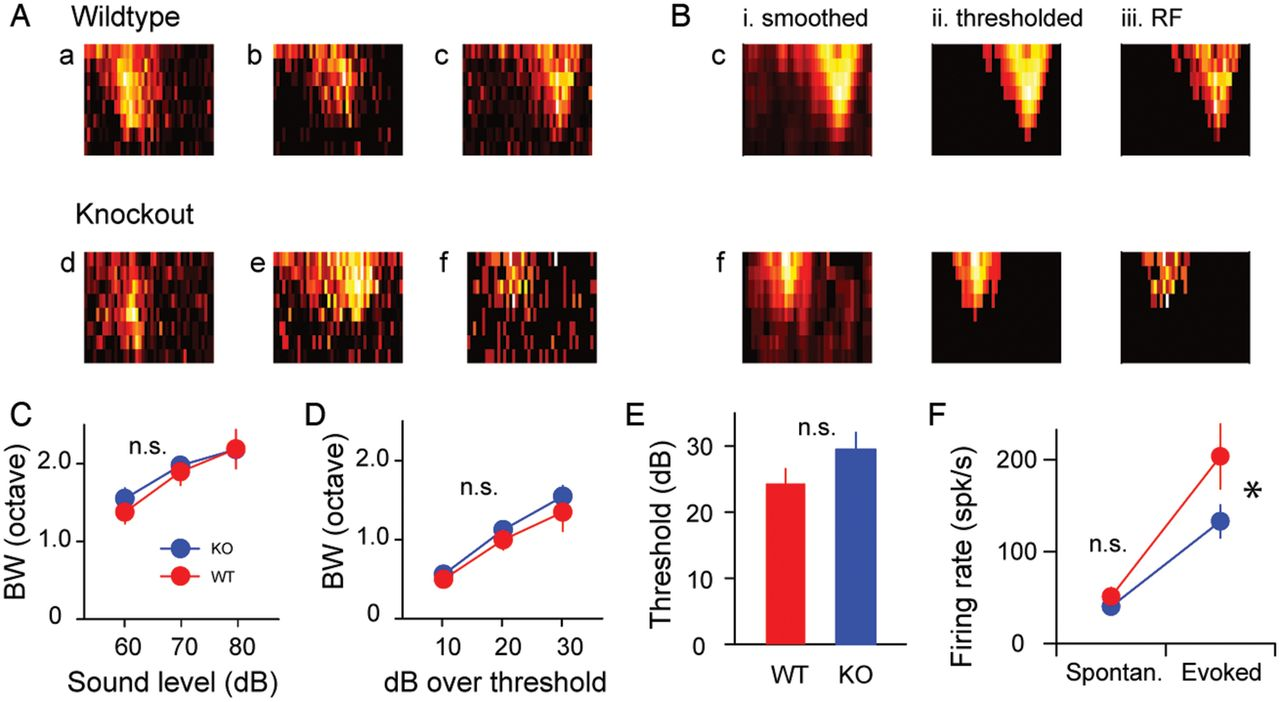
\includegraphics[width=6in]{images/C3F2}
	\begin{changemargin}{1in}{1in}
	\footnotesize{Figure 2. Cortical response properties are altered in TNF-\textalpha{} KO mice. (A) Example receptive fields recorded from WT and KO at P20. The recording sites are indicated in Figure 1. Horizontal axis depicts frequencies 4-64 kHz on a logarithmic scale. Vertical axis depicts intensity 0-70 dB with 10 dB steps. (B) Illustration of the method for automatically identifying receptive fields through smoothing and thresholding of responses in the frequency-intensity space. See Materials and Methods for details. (C and D) Tuning BWs were not altered in KO mice. (E) Stimulus threshold was not altered in KO mice. (F) Overall firing rates were reduced in KO mice. * indicates a statistically significant difference; n.s. signifies ``not significant."}
	\end{changemargin}
\end{figure}

\section{Results}

\subsection{Development of Cortical Frequency Representations Is Impaired in TNF-\textalpha{}  KO Mice}

We examined the development of sound representations in the primary auditory cortex of KO and WT mice by mapping frequency-intensity representations at three ages: postnatal day 15 (P15), P20, and P30. The basic characteristics of sound representations observed in AI of WT mice in the present study (including tonotopic organization, frequency range, tuning BW, intensity threshold, and response latency; see figures below) were consistent with those reported before (\cite{Guo2012}). By P15, the WT mice had already developed finely topographic representations of nearly the full range of frequencies from 4 to 50 kHz persisting through P30 (Fig. 1A). In contrast, the frequency map in KO mice was more variable throughout the developmental window from P15 to P30 (Fig. 1A2). AI in KO mice generally represented a narrower frequency range than that in WTs (WT, $n = 8$, 2.9 $\pm0.1$ octaves; KO, $n = 11$, $1.8\pm0.1$ octaves; ANOVA, $F_{1,17}=35.07$, $p<0.00002$) often concentrated in the middle of the hearing range (Fig. 1). In P20 animals, there were more sites representing a middle frequency range of 8-30 kHz in KO mice than WT mice (WT, 75/130; KO, 166/176; $\chi^2(1)=56.96$, $p<0.0001$; Fig. 1C).

Receptive field characterization indicated that tuning BW was not altered in KO (n = 5) compared with WT mice (n = 6; BW at 60-80 dB SPL, 2-way repeated-measures ANOVA, genotype effect $F_{1,9}=0.16$, $p=0.70$, interaction $F_{2,18}=0.48$, $p=0.63$; BW10-30, genotype, $F_{1,9}=0.56$, $p=0.47$, interaction $F_{2,18}=0.39$, $p=0.68$; Fig. 2A-D). Although KO receptive fields tended to have higher thresholds than those of WT, the effect was not significant ($F_{1,9}=3.47$, $p=0.095$; Fig. 2E). While no significant difference was found in spontaneous firing rate between WT and KO ($F_{1,9}$=2.31, $p=0.16$), the tone-evoked firing rate was significantly higher in WT than in KO mice ($F_{1,9}$=5.36, $p=0.046$; Fig. 2F).

\subsection{TNF-\textalpha{} KO Mice Exhibit Single-Frequency Exposure-Induced Map Reorganization}

We exposed both KO (n = 4) and WT (n = 4) mice to a 25-kHz tone repeated from P9 to P20, and examined sensory exposure-induced changes in cortical frequency representations. Exposure significantly increased the number of sites representing the frequency range of 25 kHz $\pm$ 0.3 octaves in both WT (na\"ive, 16/130; exposed, 68/163; $\chi^2(1)=30.59$, $p<0.0001$) and KO (na\"ive, 43/176; exposed, 70/150; $\chi^2(1)=17.68$, $p<0.0001$), indicating that KO mice undergo normal single-frequency exposure-induced map reorganization (Fig. 3). While single-frequency exposure did not alter the range of frequencies represented in AI of WT (2.9 $\pm0.2$ octaves, compared with na\"ive WT at 2.9 $\pm0.1$ octaves), it increased the AI frequency range in KO mice (2.7 $\pm0.2$ octaves, compared with na\"ive KO at 1.8 $\pm0.1$ octaves; ANOVA, $F_{3,23}=15.36$, $p<0.0001$; post-hoc: na\"ive KO vs. exposed KO, $p=0.0002$; na\"ive WTs vs. exposed WTs, $p=0.97$; na\"ive WT vs. exposed KO., $p=0.46$).

\begin{figure}[h]
	\centering
		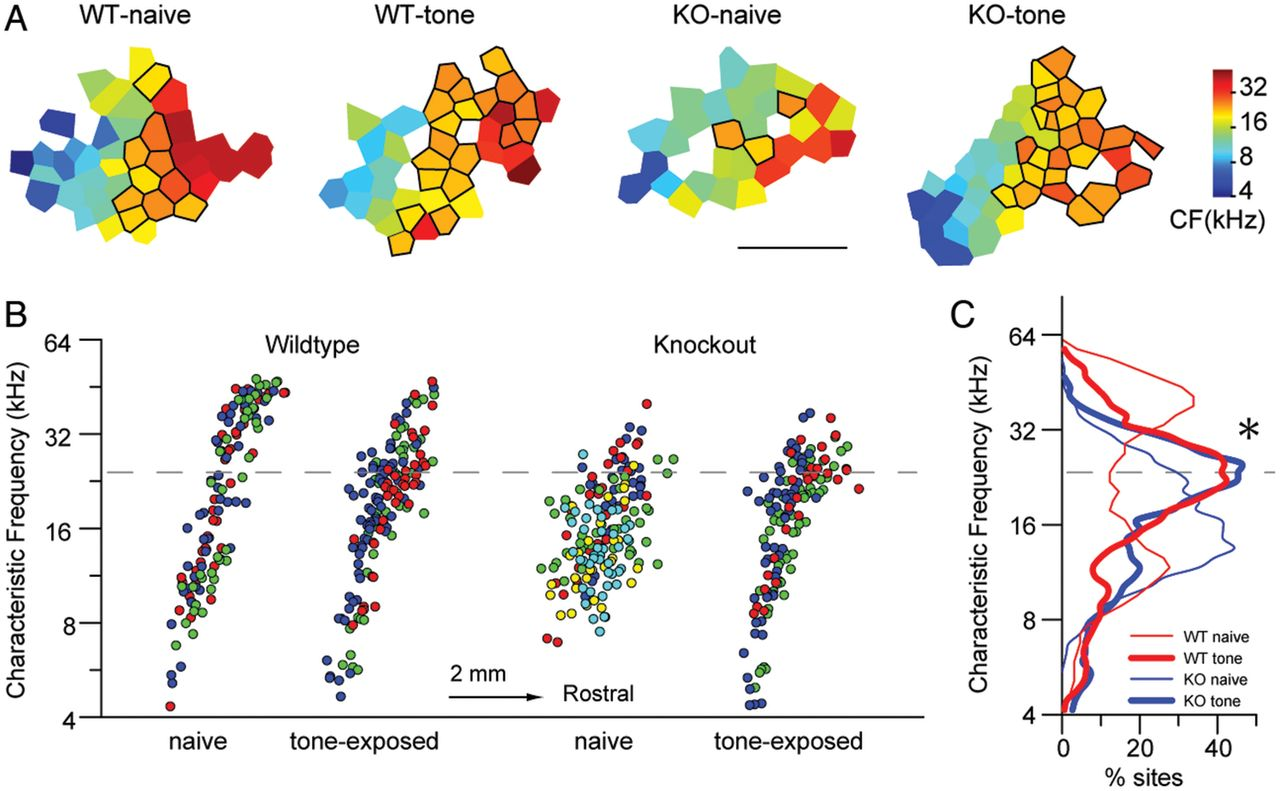
\includegraphics[width=5in]{images/C3F3}
	\begin{changemargin}{1in}{1in}
	\footnotesize{Figure 3. Single-frequency exposure-induced map reorganization is unimpaired in KO mice. (A) Example maps recorded from na\"ive and tone-exposed WT and KO mice at P20. Note the enlarged representations near 25 kHz, the exposure frequency, in exposed WT and KO animals. The scale bar is 1 mm long and applies to all maps. (B) Representative CF distributions along the rostral-caudal axis. (C) Percent of sites representing frequencies ($\pm0.3$ octaves). * indicates a statistically significant difference.}
	\end{changemargin}
\end{figure}


Single-frequency exposure had limited effects on receptive field and neuronal firing properties. Receptive field analysis indicates that single-frequency exposure did not alter overall tuning BWs of AI units (experience $\times$ genotype $\times$ intensity ANOVA with repeated measures for BW at 60-80 dB SPL, experience, $F_{1,15}=0.007$, $p=0.93$, genotype, $F_{1,15}=1.85$, $p=0.19$, interaction, $F_{1,15}=0.94$, $p=0.35$; ANOVA for BW10-30, experience, $F_{1,15}=3.29$, $p=0.09$, genotype, $F_{1,15}=3.22$, $p=0.09$, interaction, $F_{1,15}=0.003$, $p=0.96$; Fig. 4A,B). The receptive field size was not altered (genotype $\times$ experience ANOVA, genotype, $F_{1,15}=0.001$, $p=0.98$, experience, $F_{1,15}=0.18$, $p=0.90$; Fig. 4C).

We quantified mean and maximum response magnitude in the receptive field (for details, see Materials and Methods). Maximum response magnitude is the maximum number of spikes activated by any stimulus used to characterize the receptive field---that is, it measures response of a unit to its best stimulus. Mean response magnitude measures the overall responsiveness of the unit. The single-frequency exposure had different effects on KO and WT mice, enhancing responses in KO but not in WT (genotype $\times$ experience $\times$ type of response ANOVA, genotype $\times$ experience interaction, $F_{1,32}=4.15$, $p=0.0498$; Fig. 4D). We separated recorded units by their CFs---those with CFs $\ge$ 16 kHz and those with CFs $<$ 16 kHz. Neurons with CFs $\ge$ 16 kHz were more likely to be activated by the 25-kHz exposure tone than neurons with CFs $<$ 16 kHz (Fig. 3B). The maximum response magnitude was greater for tone-exposed KO mice than na\"ive KO mice only for units with high CFs (CFs $\ge$ 16 kHz) ($F_{1,7}=10.23$, $p=0.015$), but not those with low CFs (CFs $<$ 16) kHz ($F_{1,7}=1.70$, $p=0.233$). There was no difference between na\"ive and tone-exposed KO mice in mean response magnitude in either of the CF groups (CFs $\ge$ 16 kHz: $F_{1,7}=2.28$, $p=0.174$; CFs $<$ 16 kHz: $F_{1,7}=0.775$, $p=0.408$). We also separately analyzed high-CF and low-CF units recorded from na\"ive and tone-exposed WT mice, and found no significant difference in maximum or mean response magnitude (CFs $\ge$ 16 kHz: maximum response magnitude, $F_{1,8}=0.891$, $p=0.373$, mean response magnitude, $F_{1,8}=0.150$, $p=0.709$; CFs $\ge$ 16 kHz: maximum, $F_{1,8}=0.169$, $p=0.692$, mean, $F_{1,8}=0.024$, $p=0.880$).

\begin{figure}[h]
	\centering
		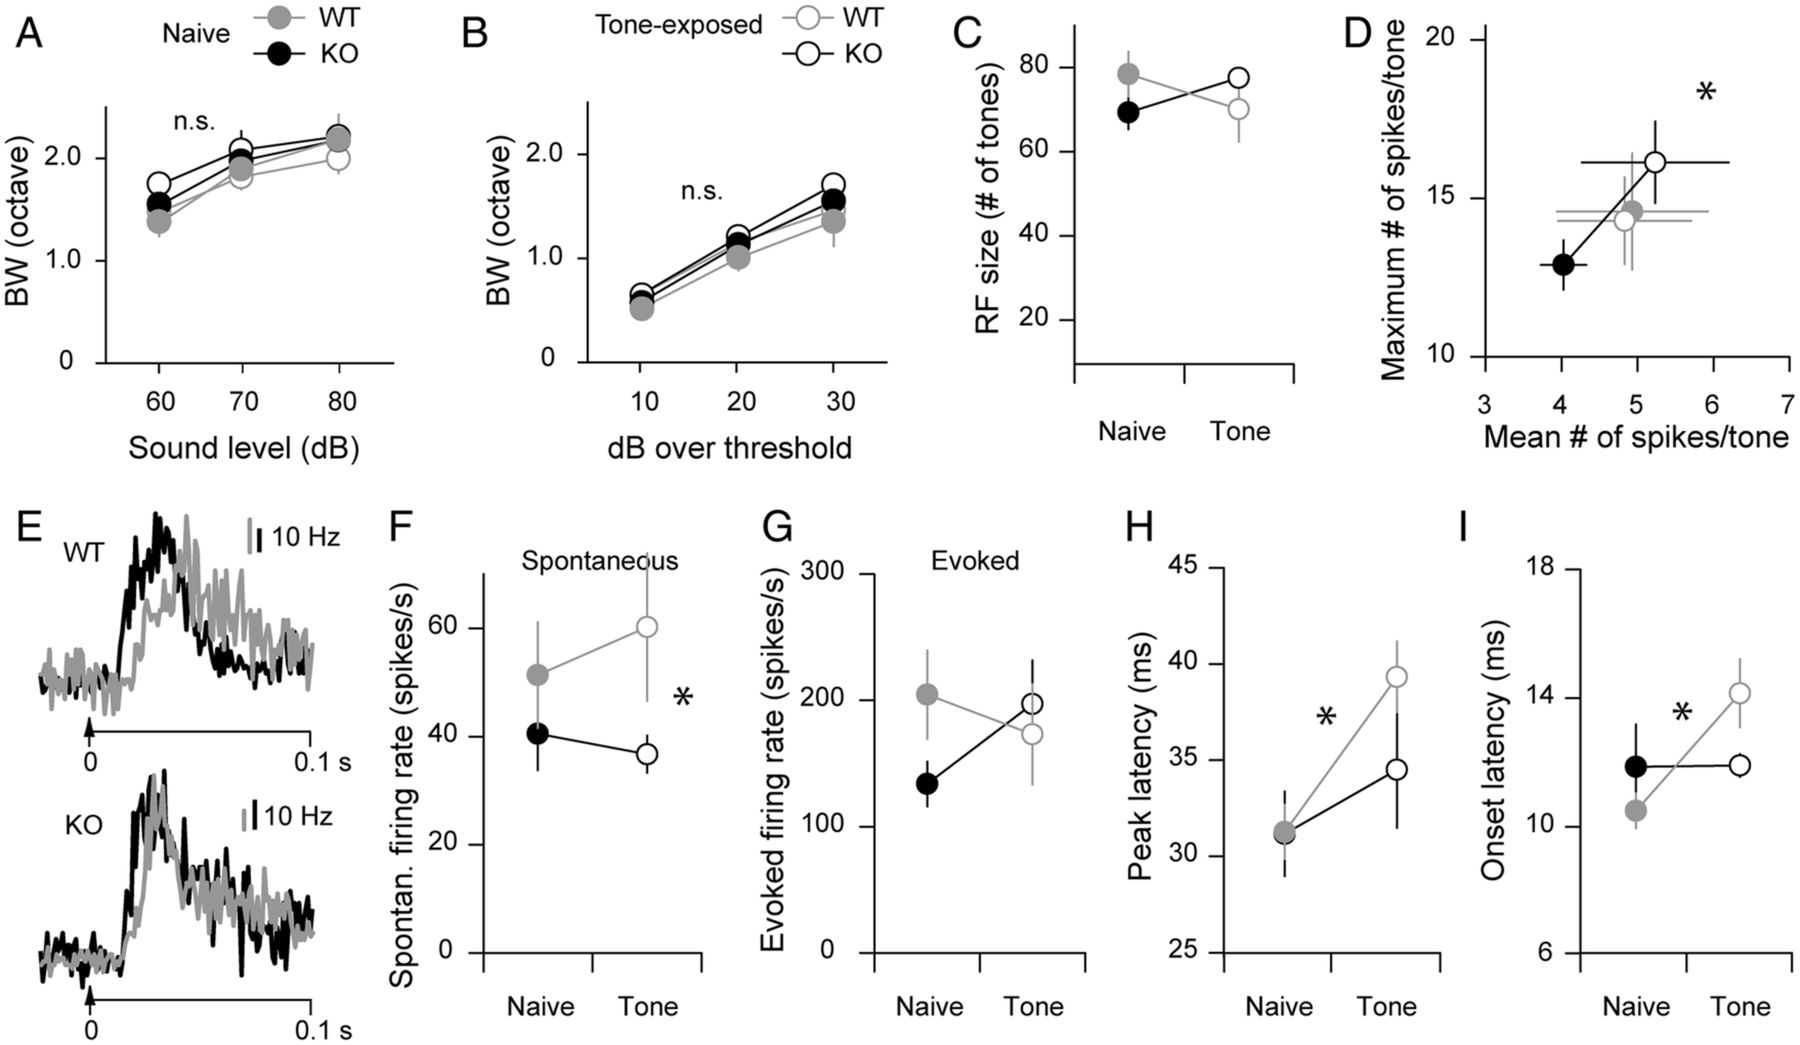
\includegraphics[width=6in]{images/C3F4}
	\begin{changemargin}{1in}{1in}
	\footnotesize{Figure 4. Effects of single-frequency exposure on cortical response properties in WT and TNF-\textalpha{} KO mice. (A-C) The single-frequency exposure did not change tuning BWs or receptive field sizes in WT or KO. (D) Mean and maximum response magnitudes to tones within the receptive field were increased in KO, but not in WT. (E) Examples of raw peri-stimulus histograms from na\"ive (black) and tone-exposed animals (gray). Note that the onset and peak of the tone-evoked responses were delayed in tone-exposed WT. (F) Although the spontaneous firing rate was generally higher in the WT than in KO, no exposure effects were observed. (G) Single-frequency exposure did not change the tone-evoked firing rate in either group. (H and I) Onset and peak latencies were increased in WT but not in KO. Asterisk indicates a statistically significant difference; n.s. signifies ``not significant."}
	\end{changemargin}
\end{figure}

We constructed PSTH with responses to all 328 (41 frequencies $\times$ 8 intensities) tone pips (Fig. 4E) to extract spontaneous and evoked firing rates, and onset and peak response latencies. Whereas the spontaneous firing rate was generally higher in WT versus KO mice (genotype $\times$ experience ANOVA, genotype effect, $F_{1,17}=5.264$, $p=0.035$; Fig. 4F), it was not altered by single-frequency exposure (experience effect, $F_{1,17}=0.048$, $p=0.83$). The tone-evoked firing rate was not different between WT and KO mice, nor between na\"ive and tone-exposed mice (genotype, $F_{1,17}=0.61$, $p=0.45$; experience, $F_{1,17}=0.47$, $p=0.50$; Fig. 4G). We also separately analyzed effects of tone-exposure for units with CFs $\ge$ 16 kHz and those with CFs $<$ 16 kHz, but did not find statistically significant differences between na\"ive and tone-exposed mice, in either WT or KO group, for either spontaneous or tone-evoked firing rates (data not shown).

Single-frequency exposure delayed the onset and peak latencies of tone-evoked responses in WT but not in KO mice (onset latency: experience, $F_{1,15}=5.70$, $p=0.031$; post-hoc WTs, $p=0.002$; KOs, $p=0.98$; Fig. 4H; peak latencies: experience, $F_{1,15}=10.87$, $p=0.0049$; post-hoc, WT, $p=0.0009$; KO, $p=0.33$; Fig. 4I). A similar finding has been reported before (\cite{Engineer2004}), but the neural mechanisms underlying the slower tone-evoked responses are unknown. Because each frequency-intensity combination was played only three times, we do not have enough data to reliably estimate onset or peak latency for individual tones.

\subsection{Multi-Frequency Exposure Refines Frequency Tuning in WT and Broadens Tuning in KO Mice}

To explore competitive interactions between different frequency inputs, we exposed WT (n = 4) and KO (n = 5) mice to an enriched multi-frequency tonal environment, in which the tone frequency was randomly chosen every 2 s from a uniform distribution ranging from 4 to 45 kHz and played in trains of 6 pips at a rate of 6 Hz. Like single-frequency exposure, our enriched environment manipulation altered the range of frequency representations (ANOVA group difference, $F_{3,24}=11.58$, $p<0.0001$; Fig. 5C,D). Post-hoc pairwise tests showed that exposure to the enriched environment expanded the represented frequency range in KO mice (compared with na\"ive KO mice, $p=0.036$), but not in WT mice ($p=0.18$). Even after exposure, the frequency range represented by KO mice was still significantly narrower than the range represented by na\"ive WT mice ($p=0.017$). However, after exposure, the representation range was no longer different between WT and KO mice ($p=0.36$).

\begin{figure}[h]
	\centering
		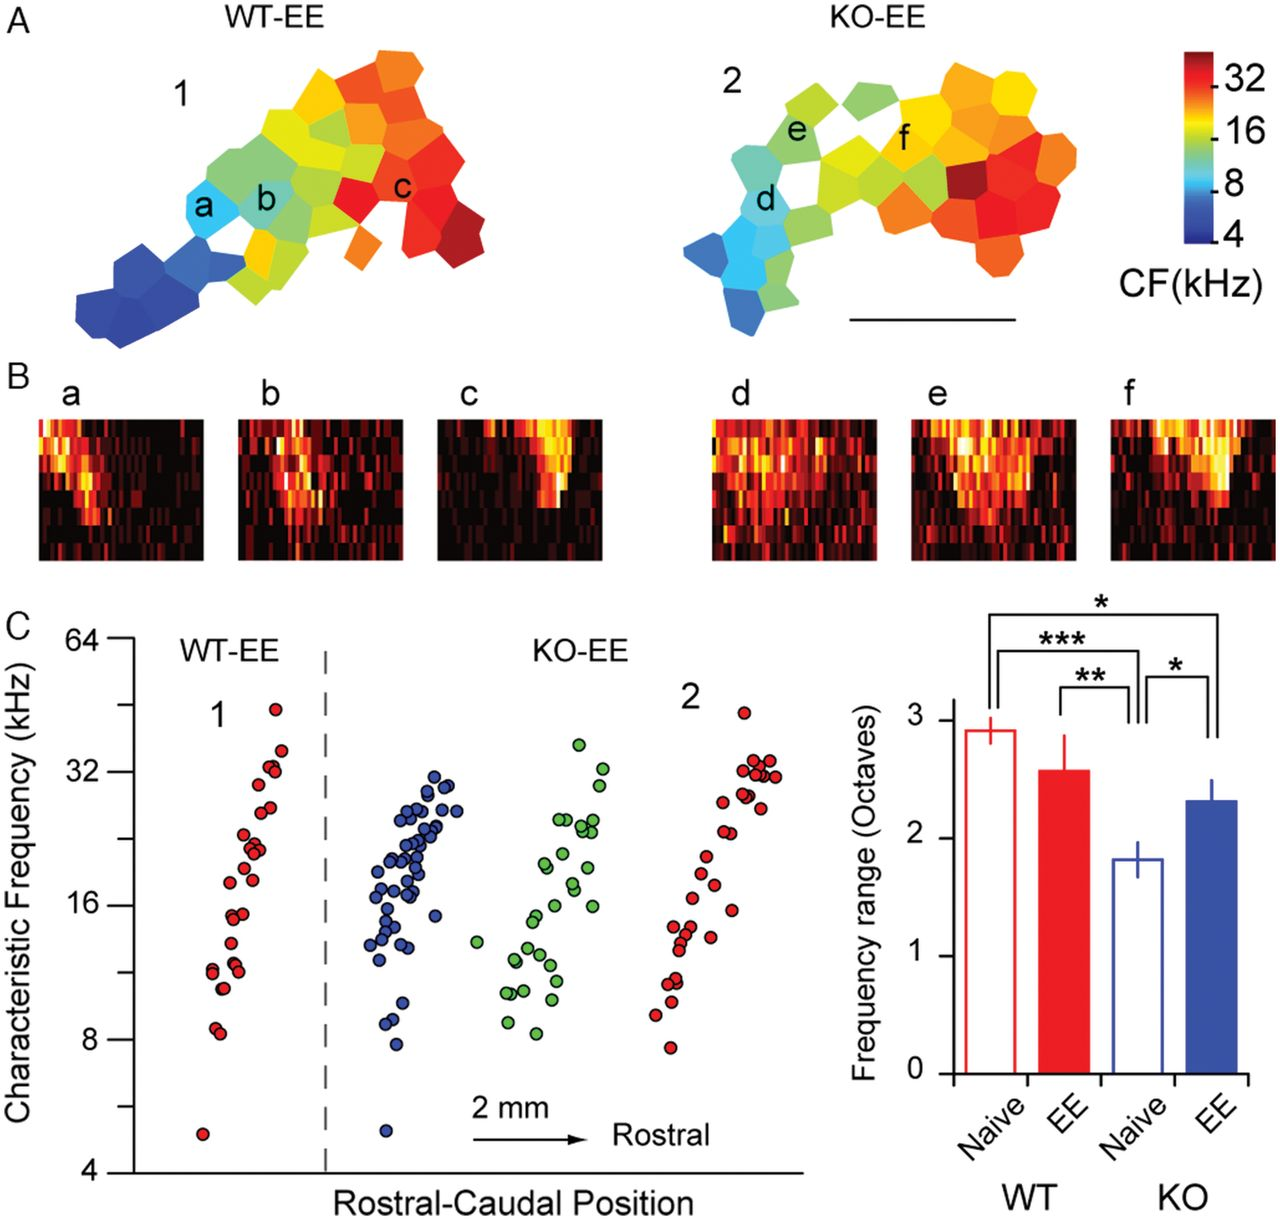
\includegraphics[width=5in]{images/C3F5}
	\begin{changemargin}{1in}{1in}
	\footnotesize{Figure 5. Multi-frequency-enriched acoustic environment increases the frequency range represented in KO mice. (A) Representative frequency maps of WT and KO mice exposed to enriched environments (EEs). (B) Representative receptive fields recorded from locations marked on cortical maps in (A). Horizontal axis: 4-64 kHz on a logarithmic scale. Vertical axis: 0-70 db SPL with 10 dB steps. (C) Representative distributions of CF on the trostral-caudal axis. Plots 1 and 2 correspond to the 2 maps in (A). (D) Frequency range represented by AI of WT and KO mice that were either na\"ive or exposed to enriched environments. *$p<0.05$; **$p<0.005$; ***$p<0.001$.}
	\end{changemargin}
\end{figure}

Exposure to the multi-frequency-enriched environment resulted in narrower frequency tuning in WT mice and broader tuning in KO mice measured at 60-80 dB SPLs (repeated-measures ANOVA, genotype $\times$ experience interaction, $F_{1,17}=15.22$, $p=0.0011$; post-hoc, exposed WT vs. all other groups, $p<0.03$; exposed KO vs. all other groups, $p<0.05$) and at 10-30 dB SPL above the threshold (interaction, $F_{1,17}=14.03$, $p=0.0016$; post-hoc, exposed KO vs. 2 WT groups, $p<0.01$; Figs 5 and 6A,B). Consistent with the altered tuning BW, we also observed reduced receptive field sizes in WT but not in KO (genotype $\times$ experience interaction, $F_{1,17}=9.17$, $p=0.0076$; post-hoc, exposed WT vs. na\"ive WT, $p=0.0048$; exposed WT vs. exposed KO, $p=0.0061$; Fig. 6C). The broadened tuning in exposed KO mice did not result in enlarged receptive field size, possibly because their threshold was slightly but not significantly increased. These results suggest that exposure to tones of different frequencies results in a winner-take-all type of competitive refinement of frequency representation in WT mice, which was impaired in KO mice lacking homeostatic plasticity.

\subsection{KO Mice Are Impaired in Homeostatic Regulation of Cortical Responses}

Overstimulation of AI with a wide range of frequencies resulted in a lower neuronal firing rate compared with na\"ive WT mice (spontaneous firing rate, $F_{1,10}=5.13$, $p=0.047$; tone-evoked, $F_{1,10}=5.71$, $p=0.038$; Fig. 6E,F), which may be considered a type of \textit{in vivo} homeostatic regulation of neuronal activity by sensory experience (see Discussion). However, exposed KO mice showed a greater tone-evoked firing rate compared with na\"ive KO mice (tone-evoked, $F_{1,8}=5.54$, $p=0.046$; Fig. 6D). Spontaneous firing rate also trended higher in the exposed KO mice, although the effect was not significant ($F_{1,8}=1.99$, $p=0.19$; Fig. 6D). A comparison of mean and maximum responses in the receptive field confirmed the above observations, showing that exposure to the multi-frequency-enriched environment lowered AI responses in WT while increasing responses in KO mice (genotype $\times$ experience $\times$ response ANOVA, experience, $F_{1,36}=4.91$, $p=0.033$; Fig. 6F). Like single-frequency exposure, the multi-frequency exposure also delayed onset and peak latencies in WT but not in KO mice (onset latency: experience, $F_{1,17}=6.36$, $p=0.022$; post-hoc WTs, $p=0.0091$; KOs, $p=0.93$; Fig. 6G; peak latencies: experience, $F_{1,17}=4.98$, $p=0.039$; post-hoc, exposed WT vs. all other groups, $p<0.04$; Fig. 6H). Instead of responding to overstimulation with a homeostatic decrease in neural activity, KO mice displayed an increase in responses indicating an absence of homeostatic processes.

\begin{figure}[h]
	\centering
		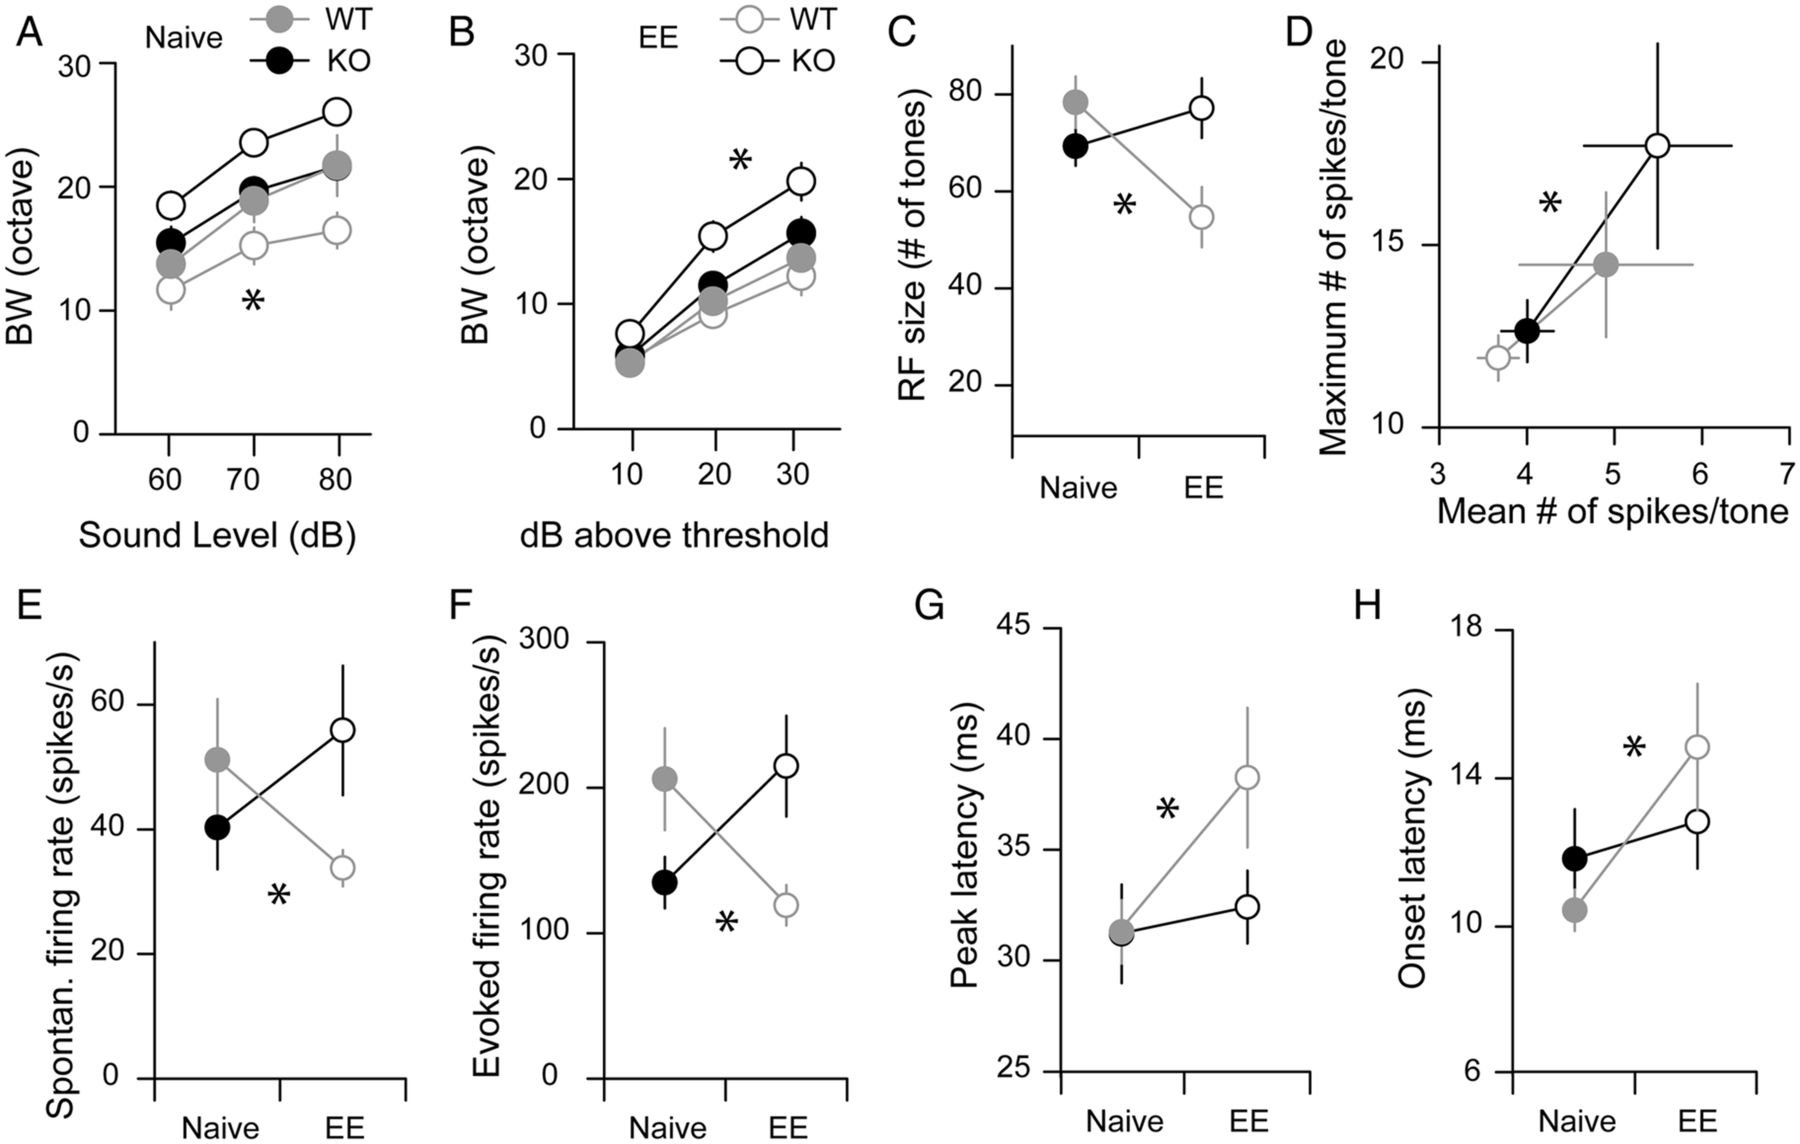
\includegraphics[width=6in]{images/C3F6}
	\begin{changemargin}{1in}{1in}
	\footnotesize{Figure 6. Effects of multi-frequency-enriched environment on cortical response properties in WT and KO mice. (A and B) Tuning BW narrowed in WT, but broadened in KO mice. (C) The receptive field size was reduced in WT, but unaltered in KO mice. (D-E) Spontaneous and tone-evoked firing rates were decreased in WT but increased in KO mice. (F) Mean and maximum response magnitudes to tones within the receptive field were increased in KO, but decreased in WT. (G and H) Onset and peak latencies were increased in WT but not in KO. Asterisk indicates a statistically significant difference.}
	\end{changemargin}
\end{figure}

\section{Discussion}

We have compared the development and sound-induced reorganization of sound representations in AI of TNF-\textalpha{} KO mice and their WT controls. Our results indicate that, compared with WT mice, KO mice 1) develop more variable and incomplete frequency representations, 2) have weaker cortical responses to tones, 3) exhibit normal expansion of cortical representations in response to single-frequency, repeated tone exposure, 4) show enhanced cortical responses after sensory over-stimulation, 5) and do not show competitive refinement of frequency representations after exposure to multi-frequency tones. These results suggest that TNF-\textalpha{} and its associated cellular processes are important in cortical response gain control and competitive refinement of cortical acoustic representations.

The mammalian auditory cortex evolved to be highly adaptive, such that it overrepresents prevalent and salient environmental sounds within the acoustic environment (\cite{Diamond1986, Gonzalez-Lima1986, Ohl1996, Pantev1998, Edeline1998, Gao2000, Zhang2001, Syka2002, Fritz2003, Mrsic-Flogel2003, Dean2005, Popescu2010, Cohen2011, Takahashi2011}). However, adaptation to some sounds may impair subsequent learning of new sounds in the future (\cite{Sarro2011}). Therefore, it is important to strike a balance between plasticity and stability. The acoustic environment can be highly variable. For example, while the acoustic environment of a typical animal room may be considered impoverished, it can be dramatically enriched locally by conspecific vocalizations (\cite{Kim2009, Grimsley2011}). Species-specific vocalizations often occur in a high-frequency range, whereas sounds in the natural environment have more power in the lower frequency range (\cite{Liu2003, Kim2009}). In addition, animals are typically more sensitive to certain frequencies in their hearing range. Experimental evidence indicates that, in spite of the environmental variability and hearing constraints, the auditory cortex more or less consistently represents a large range of hearing frequencies (e.g. see WT cortical map in Fig. 1). This stability appears to break down in TNF-\textalpha{} KO mice, which display narrower ranges and more variability in their frequency representations. This impairment seems to be the result of impoverished sensory experience, as it is reversed by repeated acoustic exposure to single or multiple tones. It is conceivable that WT animals maintain stable acoustic representations in an impoverished sensory environment by enhancing input connectivity in the understimulated sensory pathways through homeostatic mechanisms. In animals with deficient homeostatic plasticity but normal Hebbian plasticity, cortical representations may be dictated to a greater degree by the highly variable acoustic environment, leading to impaired frequency representation as we observed in KO mice. It should be noted that no differences in retinotopy or basal visual response were observed in the primary visual cortex (VI) of the TNF-\textalpha{} KO (\cite{Kaneko2008}). The different effects of TNF-\textalpha{} KO on basal stimulus representations in AI versus VI could be due to the fact that the visual stimulation is more uniform in the retinocentric visual space, whereas auditory stimulation is highly variable in the frequency space as we have discussed above.

The lack of homeostatic regulation in KO mice was also evident in the magnitude of cortical responses. Cortical responses to tone pips were weaker in na\"ive KO than in na\"ive WT mice, which again could be attributed to the acoustically impoverished housing environment. More telling evidence comes from the finding that, after repeated exposure to the multi-frequency enriched environment, cortical responses in WT mice were reduced. Presumably, this occurs through homeostatic processes, whereas cortical responses in KO mice are enhanced through Hebbian plasticity. This is also consistent with the previous findings that TNF-\textalpha{} KO mice have normal LTP (\cite{Albensi2000, Stellwagen2006, Kaneko2008}).

Refinement of neuronal connectivity requires competitive synaptic interactions, and theoretical considerations suggest that homeostatic plasticity may be involved in such interactions (\cite{Davis2001, Burrone2003, Turrigiano2004}). Recent experimental studies examined competitive interactions in TNF-\textalpha{} KO mice by blocking the activity of a subset of sensory input through monocular deprivation. The results support a role of homeostatic plasticity underlying the competitive component of ocular dominance plasticity (\cite{Kaneko2008, Ranson2012}). In the present study, we examined competitive interactions using the opposite sensory manipulation---by overstimulation of all sensory input asynchronously. In WT mice, exposure to a multi-frequency environment resulted in narrower frequency tuning, indicative of competitive refinement of sensory representations. In contrast, the identical sensory manipulation resulted in broadened tuning in mice lacking TNF-\textalpha{}, suggesting that a TNF-\textalpha{} -mediated process, presumably homeostatic plasticity, is required for the refinement of frequency selectivity observed in WT mice. Our results support a role of homeostatic plasticity in competitive refinement of sensory representations and neuronal circuits.

As we have discussed above, the more variable and incomplete frequency representations in the AI of na\"ive KOs are likely due to impaired upregulation of sensory responses in the understimulated pathways. This is consistent with the findings that TNF-\textalpha{} is required for homeostatic upregulation of excitatory synapses and downregulation of inhibitory synapses in hippocampal and cortical slices (\cite{Stellwagen2006, Kaneko2008}). Our observation of impaired competitive interaction in the overstimulated TNF-\textalpha{} KO mice suggests that over activation-induced homeostatic downregulation of excitatory synapses and/or upregulation of inhibitory synapses is disrupted in the KOs. Although electrophysiological studies indicate that TNF-\textalpha{} is not needed for homeostatic downregulation of excitatory synapses in hippocampal slices (\cite{Stellwagen2006}), it is unclear whether homeostatic upregulation of inhibitory synapses is normal in TNF-\textalpha{} KO mice. Such a mechanism can be induced by sensory overstimulation, suppressing cortical responses (\cite{Knott2002}). Furthermore, the underlying mechanisms may be different between \textit{in vivo} homeostatic plasticity following sensory stimulation and \textit{in vitro} homeostatic plasticity after neuronal stimulation. It remains to be determined whether TNF-\textalpha{} KO mice are impaired in homeostatic plasticity following sensory deprivation or overstimulation \textit{in vivo}. While TNF-\textalpha{} KO mice are impaired in some forms of homeostatic plasticity and normal in one form of LTP (\cite{Stellwagen2006, Kaneko2008}), they may well have other uncharacterized plasticity deficits that could lead to the observed impairments in the development and competitive refinement of sound representations in AI. Further characterization of different forms of synaptic plasticity in the TNF-\textalpha{} KO mice and identification of the types of synaptic plasticity involved in experience-dependent cortical development and refinement may shed new light on how TNF-\textalpha{} is involved in those processes.

In the present study, we focused on two cortical plasticity effects observed in WT mice: single-frequency exposure-induced expansion of cortical representations at the exposure frequency and multi-frequency exposure-induced reduction of cortical response magnitude (\cite{Condon1991, Zhang2001, Pienkowski2012}). Frequency map expansion appears to involve Hebbian-type, LTP-like potentiation of excitatory synapses (\cite{Froemke2007, Sun2010}). The mechanism underlying sound exposure-induced response reduction is largely unknown. We considered it a type of homeostatic regulation of cortical activity (which is different from homeostatic synpatic plasticity) purely based on its impact at the level of cortical activity. In WT mice, repetitive stimulation with multi-frequency tones is likely to increase the overall level of cortical activity. The observed reduction of sound-evoked responses should dampen activity levels, and counterbalance the overstimulation of the auditory cortical neurons. In the present study, we defined homeostatic regulation of cortical responses as a reduction of cortical responses induced by sensory overstimulation, or an enhancement of responses caused by sensory deprivation. We found that in KO mice, single-frequency exposure induced frequency map changes, but multi-frequency exposure did not cause a response reduction, suggesting a role of TNF-\textalpha{} in homeostatic regulation of cortical activity.

The normal single-frequency exposure-induced map expansion, impaired multi-frequency exposure-induced tuning refinement, and differentially regulated cortical response patterns observed in TNF-\textalpha{} KO mice indicate that multiple cellular mechanisms are at work in shaping cortical sensory representations and response properties (\cite{Bear2003, Bear2003, Burrone2003, Turrigiano2004, Dan2006, Liu2007, Wu2008, Feldman2009}). Using genetic manipulations to target-specific cellular mechanisms, we may be able to dissect the circuits and cellular mechanisms involved in physiological and pathological plasticity. For example, both Hebbian plasticity-mediated sensory map changes and homeostatic plasticity-mediated changes in spontaneous firing rate are considered potential mechanisms underlying hearing loss-induced tinnitus and phantom pain (\cite{Eggermont2006, Yang2011a}). In the next chapter, I describe the use of TNF-\textalpha{} KO mice to help clarify the specific role of homeostatic plasticity in tinnitus.

\printbibliography